\subsection{Comparison of two-point shear statistics; the two-point correlation function, mass aperture statistic and COSEBIs}

\ch{Copied this over from original comment paper - I would like to include this material somewhere in the paper - this needs work though to make it fit.... TBD}

\citet{kilbinger/etal:2013} present a detailed comparison of cosmological constraints obtained from a range of different two-point shear statistics including the shear correlation function, $\xi_\pm$, the aperture-mass dispersion, $\langle M_ {\rm ap} \rangle ^2$ \citep{schneider/etal:1998}, and the COSEBIs, $E_n$ \citep{schneider/etal:2010}.  These statistics are linearly related to the power spectrum via integrals of the form,
%
\begin{align}
%\label{eqn:integ}
& E_n =\int_0^{\infty}\frac{\d \ell \ell}{2\pi} W_n(\ell) P(\ell)\;,\\ \nonumber
& \langle M_ {\rm ap} \rangle ^2(\theta)=\int_0^{\infty}\frac{\d \ell \ell}{2\pi} U^2_\theta(\ell) P(\ell)\;,
\end{align}
%
where $W_n(\ell)$ and $U^2_\theta(\ell)$ are defined in \cite{schneider/etal:2010} and \cite{schneider/etal:1998}. The corresponding equations for $\xi_\pm$ are given in equation~\ref{eqn:xiGG}.
Figure~\ref{fig:filters} shows the integrands of these statistics 
for two cases, normalised to their maximum value, where the integrands are of the form $\ell F(\ell) P(\ell)$. For $\xi_\pm$, $P(\ell)$ is equal to the sum of the E and B-mode power spectra, motivating the development of the aperture-mass dispersion statistic, $\langle M_ {\rm ap} \rangle ^2$.  This statistic is, however, a lossy conversion and is biased by small angular separations, where blending of galaxies makes shear measurement challenging \citep{kilbinger/etal:2006}.  The COSEBIs statistic tackles both these shortcomings.  The upper two panels of figure~\ref{fig:filters} show the integrands\footnote{Note that the lower left panel of Fig. 1 in \citet{kitching/etal:2016} shows an integrated form of this function for a maximum angular separation of $100'$. However, in \citet{kilbinger/etal:2013}, the data used in \citet{kitching/etal:2016}, $\theta$ is between $0.8'$ and $350'$.} of $\xi_\pm$ for $\theta=100'$ and $\theta=350'$. The lower middle panel in Figure~\ref{fig:filters} shows the COSEBIs integrands for two angular ranges, $[1',100']$ and $[0.8',350']$, where we only show the integrands for the lowest COSEBIs mode, $E_1$, as the higher modes generally probe larger $\ell$-modes.  Finally, the lowest panel shows the integrands of aperture mass dispersion statistics, for the same two maximum angular ranges. 

\begin{figure}%[!htp]
\begin{center}
\begin{tabular}{ccc}
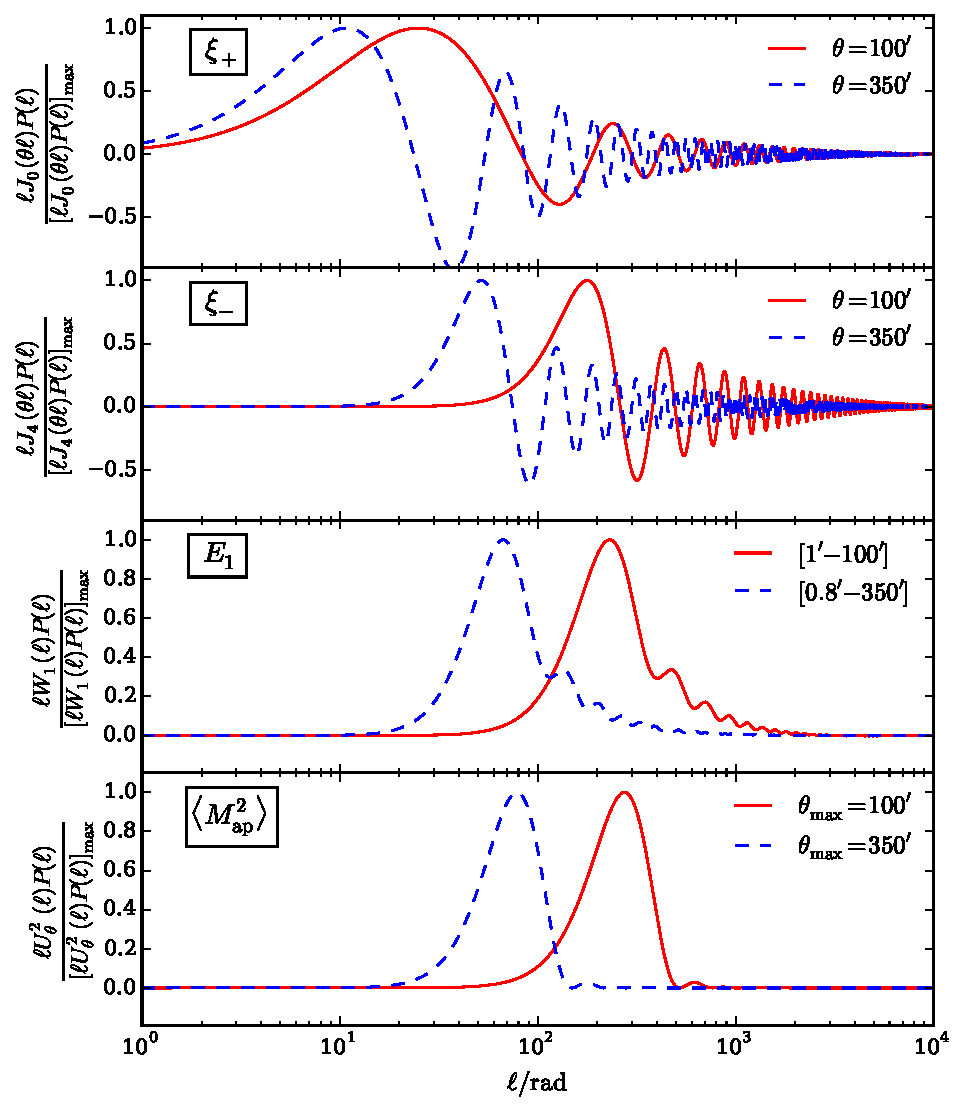
\includegraphics[width=0.48\textwidth]{figures/IntegAll.pdf} \\
\end{tabular}
\caption{ \small{\label{fig:filters}. Integrand of $\xi_+$ (upper), $\xi_-$ (upper middle), $E_1$ (lower middle, E-COSEBIs) and $\langle M_{\rm ap} \rangle^2$ (lower panel).
All integrands are of the form $\ell F(\ell) P(\ell)$, where $F(\ell)$ is the corresponding weight-function
for each statistic and $P(\ell)$ is the E-mode convergence power spectrum, with the exception of $\xi_\pm$, for which
$P(\ell)$ is equal to the sum of the E and B-mode power spectra. 
Two cases are shown for each statistic as listed in each caption.
For the aperture mass statistic $\theta_{\rm max}=2\theta$ is shown. 
Note that higher order COSEBIs modes generally probe larger $\ell$-modes, 
hence here we only show the lowest mode $E_1$. All values are normalized with respect to their maximum value. }
}
\end{center}
\end{figure}

From Figure~\ref{fig:filters} we can see that the two-point cosmic shear statistics tested by \citet{kilbinger/etal:2013} exhibit different dependences between the angular scales sampled and the $\ell$-range probed.   
If a significant bias had been introduced at low-$\ell$ by using flat-sky and Limber approximations, we would then expect to see a systematic shift between the different two-point statistics with the COSEBIs statistic being essentially unaffected as it only includes modes with $\ell \gtrsim 20$.  This is found not to be the case with all three statistics finding $\sigma_8 (\Omega_m/0.27)^\alpha = 0.79$ with errors that range from $0.03$ to $0.06$ for the full five-parameter fit, and $\alpha$ ranging from $0.59$ to 0.7 \citep[see Table 5 of][]{kilbinger/etal:2013}.  This comparison further supports our argument that the approximations highlighted by \citet{kitching/etal:2016} have negligible impact for current surveys.

